\documentclass[12pt]{article}
\usepackage{light}

\newcommand{\spa}{\spadesuit}
\newcommand{\hea}{\heartsuit}
\newcommand{\dia}{\diamondsuit}
\newcommand{\clu}{\clubsuit} 


\hidesolutions
%\showsolutions

\begin{document}

\recitation{16}{November 5, 2014}

%%%%%%%%%%%%%%%%%%%%%%%%%%%%%%%%%%%%%%%%%%%%%%%%%%%%%%%%%%%%%%%%%%%%%%%%%%%%%%%

\section{Combinatorial Proof}

A \term{combinatorial proof} is an argument that establishes an
algebraic fact by relying on counting principles.  Many such proofs
follow the same basic outline:
%
\begin{enumerate}

\item Define a set $S$.

\item Show that $\size{S} = n$ by counting one way.

\item Show that $\size{S} = m$ by counting another way.

\item Conclude that $n = m$.

\end{enumerate}

\insolutions{
Consider the following theorem:

\begin{theorem*}
\[
\sum_{i=0}^n \binom{k+i}{k} = \binom{k+n+1}{k+1}
\]
\end{theorem*}

%% We already know how to prove this theorem using induction.  Here's
%% how we would do it:
%% 
%% \vspace{0.5in}
%% 
%% \begin{proof}
%% The proof is by induction on $n$. Let $P(n)$ be the proposition that $\forall
%% k>0$, $\sum_{i=0}^n \binom{k+i}{k}=\binom{k+n+1}{k+1}, n\geq 0$.
%% 
%% {\bf Base case:} $P(0)$ is true because
%% 
%% \[
%% \forall k>0, \sum_{i=0}^0 \binom{k+i}{k}=\binom{k}{k}=\binom{k+1}{k+1}=1
%% \]
%% 
%% {\bf Inductive step:} Assume $P(n)$ is true. Show $P(n+1)$ must be
%% true $\forall n>0$.
%% 
%% \begin{align}
%% \forall k>0, \sum_{i=0}^{n+1} \binom{k+i}{k} &= \binom{k+n+1}{k} + \sum_{i=0}^n \binom{k+i}{k}\\
%% &= \binom{k+n+1}{k} + \binom{k+n+1}{k+1}\label{ih}\\
%% &= \frac{(k+n+1)!}{k!(n+1)!} + \frac{(k+n+1)!}{(k+1)!n!}\label{def}\\
%% &= \frac{(k+1)(k+n+1)! + (k+n+1)!(n+1)}{(k+1)!(n+1)!}\\
%% &= \frac{(k+n+1)!(k+n+2)}{(k+1)!(n+1)!}\\
%% &= \frac{(k+n+2)!}{(k+1)!(n+1)!}\\
%% &= \binom{k+n+2}{k+1}
%% \end{align}
%% 
%% The inductive hypothesis is applied in Step~\ref{ih}. Step~\ref{def}
%% follows by definition of choose, and the remaining steps are algebraic
%% simplifications.
%% \end{proof}
%% 
%% \vspace{0.5in}
%% 
%% How messy!  A combinatorial proof would be simpler:

%% Give a
%% combinatorial proof of the theorem.  For this problem, let $S$ be
%% the set of all binary sequences with exactly $n$ zeroes and $k + 1$
%% ones.
%% 
%% Hint: look at the number of zeroes to the left of the rightmost one.

%\solution[\vspace{1in}]{
%\begin{proof}
%We give a combinatorial proof.  Let $S$ be the set of all sequences in
%$\set{0, 1, *}^n$ containing exactly one $*$.
%
%On one hand, $\size{S} = n 2^{n-1}$, since the $*$ can appear in $n$
%positions and there are $2^{n-1}$ settings for the remaining symbols.
%
%On the other hand, every sequence in $S$ contains between 1 and $n$
%nonzero entries since the $*$, at least, is nonzero.  The number of
%sequences in $S$ with exactly $k$ nonzero entries is $k \binom{n}{k}$,
%since there are $\binom{n}{k}$ ways to select the positions of the
%nonzero entries and then $k$ ways to select one of those entries to be
%the $*$.  Thus, by the Sum Rule:
%%
%\[
%\size{S} = \sum_{k=1}^n k \binom{n}{k}
%\]
%%
%Equating these two expressions for $\size{S}$ proves the theorem.
%\end{proof}
%}
%\solution[\vspace{1in}]{

We can prove it with a combinatorial approach:

\begin{proof}
We give a combinatorial proof.  Let $S$ be the set of all binary
sequences with exactly $n$ zeroes and $k + 1$ ones.

On the one hand, we know from a previous recitation that the number of
such sequences is equal to $\binom{k + n + 1}{k+1}$.

On the other hand, the number of zeroes $i$ to the left of the rightmost
one ranges from 0 to $n$.  For a fixed value of $i$, there are
$\binom{k + i}{k}$ possible choices for the sequence of bits before the
rightmost one.  If we sum over all possible $i$, we find that
$|S| = \sum_{i = 0}^n \binom{k + i}{k}$.

Equating these two expressions for $\size{S}$ proves the theorem.
\end{proof}
} % end insolutions
%}


%%%%%%%%%%%%%%%%%%%%%%%%%%%%%%%%%%%%%%%%%%%%%%%%%%%%%%%%%%%%%%%%%%%%%%%%%%%%%%%

\section{Triangles}
Let $T=\{X_1,\ldots, X_t\}$ be a set whose elements $X_i$ are themselves
sets such that each $X_i$ has size 3 and is $\subseteq \{1,2,\ldots, n\}$.
We call the elements of $T$ ``triangles''. Suppose that for all
``edges'' $E\subseteq \{1,2,\ldots, n\}$ with $|E|=2$ there are exactly
$\lambda$ triangles $X\in T$ with $E\subseteq X$.

For example, if we might have the triangles depicted in the following
diagram, which has $\lambda = 2$, $n = 4$, and $t = 4$:

\begin{center}
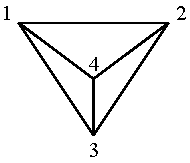
\includegraphics[height=1.5in]{triangles2}
\end{center}

In this example, each edge appears in exactly two of the following triangles:

$$\{1, 2, 3\}, \{1, 2, 4\}, \{1, 3, 4\}, \{2, 3, 4\}$$

Prove
$$ \lambda \cdot \frac{n(n-1)}{2} = 3t$$
by counting the set
$$C= \{ (E,X) : X\in T, E\subseteq X, |E|=2\}$$
in two different ways.

\solution[\vspace{1.5in}]{
We give a combinatorial proof.  Let $C$ be
$\{ (E,X) : X\in T, E\subseteq X, |E|=2\}$.

On the one hand, there are ${n \choose 2}$ sets $E\subseteq \{1,\ldots, n\}$
of size $|E|=2$. For each such $E$ there are exactly $\lambda$
triangles $X\in T$ with $E\subseteq X$. So,
$|C|=\lambda {n \choose 2} = \lambda \cdot \frac{n(n - 1)}{2}$.

On the other hand, there are $t$ triangles. Each triangle has exactly
${3 \choose 2}=3$
subsets $E$ of size 2. So, $|C|=3t$.

Equating these two expressions for $|C|$ proves the theorem.
}

\iffalse
%%%%%%%%%%%%%%%%%%%%%%%%%%%%%%%%%%%%%%%%%%%%%%%%%%%%%%%%%%%%%%%%%%%%%%%%%%%%%%%
\insolutions{


\section{The trick, revealed!}

Just to remind you of yesterday's magic trick:


There is a Magician and an Assistant.  The Assistant goes into the
audience with a deck of 52 cards while the Magician looks away.  Five
audience members each select one card from the deck.  The Assistant
then gathers up the five cards and reveals four of them to the
Magician, one at a time.  The Magician concentrates for a short time
and then correctly names the secret, fifth card!

\subsection{The Secret}

The Assistant somehow communicated the secret card to the Magician
just by naming the other four cards.  In particular, the Assistant has
two ways to communicate:

\begin{enumerate}

\item He can announce the four cards in any order.  The number of
orderings of four cards is $4! = 24$, so this alone is insufficient to
identify which of the remaining 48 cards is the secret one.

\item The Assistant can choose which four of the five cards to reveal.
Of course, the Magician can not determine which of these five
possibilities the Assistant selected since he does not know the secret
card.


\end{enumerate}

\noindent Nevertheless, these two forms of communication allow the
Assistant to covertly reveal the secret card to the Magician.
Remember that the trick needs to be fairly simple, since
the Magician and the Assistant need to be able to
remember how to do it under pressure (and yesterday, the Magician couldn't
even remember how many cards to choose).

%Let $X$ be a collection of all the \textit{sets} of 5 cards.
%Let $Y$ be all the sequences of 4 distinct cards.  
As an running
example, suppose that the audience selects:
%
\[
10 \hea \quad 9 \dia \quad 3 \hea \quad Q \spa \quad J \dia
\]

\begin{itemize}

\item The Assistant picks out two cards of the same suit.  In the
example, the assistant might choose the $3 \hea$ and $10 \hea$.

\item The Assistant locates the values of these two cards on the cycle
shown below:

\begin{center}
\begin{picture}(120,120)(-60,-60)
% \put(-60,-60){\framebox(120,120){}} % bounding box
\put(0.000000,50.000000){\makebox(0,0){$A$}}
\put(23.236159,44.272801){\makebox(0,0){$2$}}
\put(41.149193,28.403237){\makebox(0,0){$\mathbf{3}$}}
\put(49.635444,6.026834){\makebox(0,0){$4$}}
\put(46.750812,-17.730244){\makebox(0,0){$5$}}
\put(33.156133,-37.425537){\makebox(0,0){$6$}}
\put(11.965783,-48.547091){\makebox(0,0){$7$}}
\put(-11.965783,-48.547091){\makebox(0,0){$8$}}
\put(-33.156133,-37.425537){\makebox(0,0){$9$}}
\put(-46.750812,-17.730244){\makebox(0,0){$\mathbf{10}$}}
\put(-49.635444,6.026834){\makebox(0,0){$J$}}
\put(-41.149193,28.403237){\makebox(0,0){$Q$}}
\put(-23.236159,44.272801){\makebox(0,0){$K$}}
\end{picture}
\end{center}

For any two distinct values on this cycle, one is always between 1 and
6 hops clockwise from the other.  For example, the $3 \hea$ is 6 hops
clockwise from the $10 \hea$.

\item The more counterclockwise of these two cards is revealed first,
and the other becomes the secret card.  Thus, in our example, the $10
\hea$ would be revealed, and the $3 \hea$ would be the secret card.
Therefore:

\begin{itemize}

\item The suit of the secret card is the same as the suit of the first
card revealed.

\item The value of the secret card is between 1 and 6 hops clockwise
from the value of the first card revealed.

\end{itemize}

\item All that remains is to communicate a number between 1 and 6.
The Magician and Assistant agree beforehand on an ordering of all the
cards in the deck from smallest to largest such as:
%
\[
A \clu\ 2 \clu\ \ldots\ K \clu\ 
A \dia\ 2 \dia\ \ldots\ Q \dia\ 
A \hea\ 2 \hea\ \ldots\ Q \hea\ 
A \spa\ 2 \spa\ \ldots\ Q \spa
\]
%
The order in which the last three cards are revealed communicates the
number according to the following scheme:
%
\[
\begin{array}{rcccll}
(&\text{small},&\text{medium},&\text{large}&) & = 1 \\
(&\text{small},&\text{large},&\text{medium}&) & = 2 \\
(&\text{medium},&\text{small},&\text{large}&) & = 3 \\
(&\text{medium},&\text{large},&\text{small}&) & = 4 \\
(&\text{large},&\text{small},&\text{medium}&) & = 5 \\
(&\text{large},&\text{medium},&\text{small}&) & = 6
\end{array}
\]
%
In the example, the Assistant wants to send 6 and so reveals the
remaining three cards in large, medium, small order.  Here is the
complete sequence that the Magician sees:
%
\[
10 \hea \quad Q \spa \quad J \dia \quad 9 \dia
\]

\item The Magician starts with the first card, $10 \hea$, and hops 6
values clockwise to reach $3 \hea$, which is the secret card!

\end{itemize}
}
\fi



\section{Counting, counting, counting}
Learning to count takes practice!  Briefly justify your answers to the
following questions.  Not every problem can be solved with a cute
formula; you may have to fall back on case analysis, explicit
enumeration, or ad hoc methods.  Do as many problems as you can and
save the rest to study for Quiz II.  You may leave factorials and
binomial coefficients in your answers.

\begin{enumerate}
\item How many different arrangements are there of the letters in
$BANANA$?

\solution[\vspace{1in}]{
By the Bookkeeper Rule, there are:
%
\[
\frac{6!}{1! \ 3! \ 2!} = 60
\]
}

\item How many different paths are there from point $(0, 0, 0)$
to point $(10, 20, 30)$ if every step increments one coordinate and
leaves the other two unchanged?

\solution[\vspace{1in}]{There is a bijection between the set of all
such paths and the set of strings containing 10 X's, 20 Y's, and 30
Z's.  In particular, we obtain a path by working through a string from
left to right.  An $X$ corresponds to a step that increments the first
coordinate, a $Y$ increments the second coordinate, and a $Z$
increments the third.  The number of such strings is:

\[
\frac{60!}{10!\ 20!\ 30!}
\]

\noindent Therefore, this is also the number of paths.
}

%\item In how many different ways can $2n$ students be paired
%up?
%
%\solution[\newpage]{Pair up students by the following procedure.
%Line up the students and pair the first and second, the third and
%fourth, the fifth and sixth, etc.  The students can be lined up in
%$(2n)!$ ways.  However, this overcounts by a factor of $2^n$, because
%we would get the same pairing if the first and second students were
%swapped, the third and fourth were swapped, etc.  Furthermore, we are
%still overcounting by a factor of $n!$, because we would get the same
%pairing even if pairs of students were permuted, e.g., the first and
%second were swapped with the ninth and tenth.  Therefore, the number
%of pairings is:
%
%\[
%\frac{(2n)!}{2^n \cdot n!}
%\]
%}
%
%\item How many different nonnegative integer solutions are there to the
%following equation?
%%
%\[
%x_1 + x_2 + x_3 + \ldots + x_{10} = 1000
%\]
%
%Two solutions are different if different values are specified for some
%variable $x_i$.
%
%\solution[\vspace{1in}]{There is a bijection between strings
%containing 1000 zeros and 9 ones and solutions to this equation.  The
%9 ones divide the zeros into 10 segments.  Let $x_i$ be the number of
%zeros in the $i$-th segment.  Therefore, the number of solutions is:
%
%\[
%\binom{1000+9}{9}
%\]
%}
%
%\item How many different size $n$ subsets are there of a set $2n$
%objects, given that $n$ of the $2n$ objects are identical and the other
%$n$ are all unique?
%
%\solution[\vspace{1in}]{We can select a size $n$ subset as follows.
%First, take a subset of the unique objects.  Then take however many
%identical elements are needed to bring the total to $n$.  The first step
%can be done in $2^n$ ways, and the second can be done in only 1 way.
%Therefore, there are $2^n$ ways to choose $n$ objects.
%}
%
%\item How many undirected graphs without self-loops are there
%with vertices $v_1, v_2, \ldots, v_n$?
%
%\solution[\vspace{1in}]{There are $\binom{n}{2}$ potential edges, each
%of which may or may not appear in a given graph.  Therefore, the
%number of graphs is:
%%
%\[
%2^{\binom{n}{2}}
%\]
%}
%
\iffalse
\item A shelf holds 12 books in a row.  How many ways are there to
choose five books so that no two adjacent books are chosen?

\solution[\vspace{1in}]{There exists a bijection from 8-bit sequences
with exactly five 1's to valid book selections.  Map each zero to a
non-chosen book, each of the first four 1's to a chosen book followed
by a non-chosen book, and the last 1 to a chosen book.  For example,
the 8-bit sequence:
%
\[
(1, 0, 1, 1, 0, 1, 0, 1)
\]
%
maps to the book selection:
%
\[
\underbrace{c\ n}_{1}\ 
\underbrace{n}_{0}\ 
\underbrace{c\ n}_{1}\ 
\underbrace{c\ n}_{1}\ 
\underbrace{n}_{0}\ 
\underbrace{c\ n}_{1}\ 
\underbrace{n}_{0}\ 
\underbrace{c}_{1}
\]
%
where $c$ denotes a chosen book and $n$ denotes a non-chosen book.
Therefore, the number of valid book selections is $\binom{8}{5}$.}
\fi

\item Find the number of 5-card hands with exactly three aces.

\solution[\vspace{1in}]{We can choose the three aces in $\binom{4}{3}$
ways, and we can choose the remaining two cards in $\binom{48}{2}$
ways.  Thus, there are $\binom{4}{3} \binom{48}{2}$ such hands.}

\item Find the number of 5-card hands in which every suit
appears at most twice.

\solution[\vspace{1in}]{There are two cases.  Either one suit appears
twice or else two suits appear twice.  The number of hands in which
one suit appears twice is $\binom{13}{2} \cdot 13^3 \cdot 4$, since
there are 4 ways to choose the doubly represented suit,
$\binom{13}{2}$ ways to choose two values from this suit, and $13^3$
ways to choose values for cards in the three remaining suits.
Similarly, the number of hands in which two suits appear twice is
$\binom{13}{2}^2 \cdot 13 \cdot \binom{4}{2} \cdot 2$.  Therefore,
there are a total of
%
\[
\binom{13}{2} \cdot 13^3 \cdot 4 + \binom{13}{2}^2 \cdot 13 \cdot \binom{4}{2} \cdot 2
\]
%
such hands.}

\item There are 15 sidewalk squares in a row.  Suppose that a ball is
thrown down the row so that it bounces on 0, 1, 2, or 3 distinct sidewalk
squares.  How many different throws are possible?  Two throws are
considered to be equivalent if they bounce on the same squares in a
different order.

\solution[\vspace{1in}]{
\[
\binom{15}{0} + \binom{15}{1} + \binom{15}{2} + \binom{15}{3}
\]
}

%\item Find the number of 7-card hands with three pairs and no three-
%or four-of-a-kind.
%
%\solution[\vspace{1in}]{We can select the values of the three pairs in
%$\binom{13}{3}$ ways, the suits for the three pairs in
%$\binom{4}{2}^3$ ways, and the final card in 40 ways.  This gives:
%
%\[
%40 \binom{13}{3} \binom{4}{2}^3
%\]
%
%hands in all.}
%
\item In how many different ways can the numbers shown on a red
die, a green die, and a blue die total up to 15?  Assume that these
are ordinary, 6-sided dice.

\solution[\vspace{1in}]{We fall back on explicit enumeration.  Let
$R$, $G$, and $B$ be the values shown on the three dice.
\[\begin{array}{rlrlcl}
R & = 1, & B + G & = 14 & \rightarrow  0 \ \text{ways} \\
R & = 2, & B + G & = 13 & \rightarrow  0 \ \text{ways} \\
R & = 3, & B + G & = 12 & \rightarrow  1 \ \text{ways} \\
R & = 4, & B + G & = 11 & \rightarrow  2 \ \text{ways} \\
R & = 5, & B + G & = 10 & \rightarrow  3 \ \text{ways} \\
R & = 6, & B + G & = 9 & \rightarrow   4 \ \text{ways}
\end{array}\]
A total of 10 ways.

Another approach (suggested by a student in recitation) begins by
observing that the number of ways the dice can sum to 15 is the same as
the number of positive integer solutions to the equation
\[
x_1 + x_2 + x_3 = 15
\]
such that $x_i\leq 6$.  In general, counting solutions with inequality
constraints on the variables involves a tedious case analysis, but in this
case there's a trick to remove the constraints: let $y_i = 6 - x_i$.  Now
the number of desired $x_i$ solutions is the same as the number of
nonnegative integer solutions to
\begin{equation}\label{y3}
y_1 + y_2 + y_3 = 3
\end{equation}
such that $y_i \leq 5$.  But since the sum of the $y_i$'s must be three,
the constraint that $y_i \leq 5$ will be met by every nonnegative integer
solution to~\eqref{y3}.  So we need only count the number of nonnegative
integer solutions to~\eqref{y3}, which we already know is the same as the
number of binary sequences of two zeros and three ones, namely
\[
\binom{2+3}{3} =10.
\]
}

\item In how many ways can 20 indistinguishable pre-frosh be stored
in four different crates if each crate must contain an \textit{even}
number of pre-frosh?

\solution[\vspace{1in}]{There is a bijection from 13-bit strings with
exactly 3 ones. In particular, the string $0^a10^b10^c10^d$
corresponds to to storing $2a$ prefrosh in the first crate, $2b$ in
the second, $2c$ in the third, and $2d$ in the fourth.  Therefore, the
number of ways to store the pre-frosh is equal to the number of 13-bit
strings with exactly 3 ones, which is $\binom{13}{3}$.}

\item How many paths are there from point $(0, 0)$ to $(50, 50)$ if
every step increments one coordinate and leaves the other unchanged
and there are impassable boulders sitting at points $(10, 10)$ and
$(20, 20)$?

\solution[\vspace{1in}]{We use inclusion-exclusion.  The total
number of paths is $\binom{100}{50}$, but we must subtract off the
obstructed paths.  There are $\binom{20}{10} \cdot \binom{80}{40}$
paths through the first boulder, since there are $\binom{20}{10}$
paths from the start to the boulder and $\binom{80}{40}$ paths from
the boulder to the finish.  Similarly, there are $\binom{40}{20} \cdot
\binom{60}{30}$ paths through the second boulder.  However, we must
add back in paths going through both boulders, and there are
$\binom{20}{10} \cdot \binom{20}{10} \cdot \binom{60}{30}$ of those.
Therefore, the total number of paths is:
%
\[
\binom{100}{50}
- \binom{20}{10} \cdot \binom{80}{40}
- \binom{40}{20} \cdot \binom{60}{30}
+ \binom{20}{10} \cdot \binom{20}{10} \cdot \binom{60}{30}
\]
}

\item In how many ways can the 180 students in 6.042 be divided into
36 groups of 5?

%\solution[\vspace{1in}]{There is a $18!$-to-1 mapping from sequences
%containing five $1$'s, five $2$'s, \dots, and five $18$'s.
%Specifically, the sequence $(t_1, \dots, t_{90})$ corresponds to the
%assignment where each student $i$ is placed in group $t_i$.  The
%mapping is $18!$-to-1, because we can permute the team numbers (in
%$18!$ different ways) without altering the way the class is
%partitioned.  Therefore, the number of ways to divide the class into
%teams is:
%\[
%\frac{90!}{(5!)^{18} 18!}
%\]
%}
\solution[\vspace{1in}]{We can group the students using the following
procedure: line up the students in some order.  Group the first five
students, the sixth through tenth students, the eleventh through
fifteenth students, and so on.  The students can be lined up in 180!
ways.  However, this overcounts by a factor of $(5!)^{36}$, since the
students within each of the 36 groups can be ordered in 5! ways.  We
are also overcounting by an additional factor of 36!, since the 36
groups can be ordered in 36! ways.  Thus, the number of groupings is
\[\frac{180!}{(5!)^{36} \cdot 36!} \]
}

\item In how many different ways can 10 indistinguishable balls be
placed in four distinguishable boxes, such that every box gets 1, 2,
3, or 4 balls?

\solution[\vspace{1in}]{First, we might as well put 1 ball in every
box.  Now the problem is to put the remaining 6 balls into 4 boxes so
that no box gets more than 3 balls.  Now we turn to case analysis.
For example, we could put 3 balls in two boxes and 0 balls in the
other two boxes.  There are $4!/(2!\ 2!) = 6$ ways to do this.  All
cases are listed below:
\[
\begin{array}{ccl}
\text{distribution of balls} & \text{\# of ways} \\
3, 3, 0, 0 & \dfrac{4!}{2!\ 2!} & = 6\\
3, 2, 1, 0 & \dfrac{4!}{1!\ 1!\ 1!\ 1!} & = 24 \\
3, 1, 1, 1 & \dfrac{4!}{3!\ 1!} & = 4 \\
2, 2, 2, 0 & \dfrac{4!}{3!\ 1!} & = 4 \\
2, 2, 1, 1 & \dfrac{4!}{2!\ 2!} & = 6\\
\end{array}
\]
}

\item In how many different ways can Blockbuster arrange 64 copies of
{\em Cat in the Hat}, 96 copies of {\em Matrix Revolutions}, and 1
copy of {\em Amelie} on 5 shelves?

\solution[\vspace{1in}]{This is the number of ways to arrange 64 $C$'s
(Cat in the Hat), 96 $M$'s (Matrix), 1 $A$'s (Amelie), and 4 $X$'s
(dividers between shelves).  This is equal to:
%
\[
\frac{(64 + 96 + 1 + 4)!}{64!\ 96!\ 1!\ 4!}
\]
}

\end{enumerate}


\section{There's more than one way...}

In the beginning of today's recitation, we gave a combinatorial proof
of the following theorem:

\begin{theorem*}
\[
\sum_{i=0}^n \binom{k+i}{k} = \binom{k+n+1}{k+1}
\]
\end{theorem*}

We can also prove this theorem using induction. Give such a proof.

\solution{
\vspace{0.5in}

\begin{proof}
The proof is by induction on $n$. Let $P(n)$ be the proposition that $\forall
k>0$, $\sum_{i=0}^n \binom{k+i}{k}=\binom{k+n+1}{k+1}, n\geq 0$.

{\bf Base case:} $P(0)$ is true because

\[
\forall k>0, \sum_{i=0}^0 \binom{k+i}{k}=\binom{k}{k}=\binom{k+1}{k+1}=1
\]

{\bf Inductive step:} Assume $P(n)$ is true. Show $P(n+1)$ must be
true $\forall n>0$.

\begin{align}
\forall k>0, \sum_{i=0}^{n+1} \binom{k+i}{k} &= \binom{k+n+1}{k} + \sum_{i=0}^n \binom{k+i}{k}\\
&= \binom{k+n+1}{k} + \binom{k+n+1}{k+1}\label{ih}\\
&= \frac{(k+n+1)!}{k!(n+1)!} + \frac{(k+n+1)!}{(k+1)!n!}\label{def}\\
&= \frac{(k+1)(k+n+1)! + (k+n+1)!(n+1)}{(k+1)!(n+1)!}\\
&= \frac{(k+n+1)!(k+n+2)}{(k+1)!(n+1)!}\\
&= \frac{(k+n+2)!}{(k+1)!(n+1)!}\\
&= \binom{k+n+2}{k+1}
\end{align}

The inductive hypothesis is applied in Step~\ref{ih}. Step~\ref{def}
follows by definition of choose, and the remaining steps are algebraic
simplifications.
\end{proof}
\vspace{0.5in} 

It is always good to have more than one way to solve a problem!
}

\end{document}
